\chapter{Future Work}
\label{Future}

% LONDON install and experiments
%  MMR install
% CLinical comparison 
% SPECT MR study 
% NEW calibration procedure 
% Image Registration 
% SIMIND 
% Alternative Hardware 
% Alt. Use (Epilepsy, Foot, Bedside SPECT, cheap system ) 


% Clinical comparison with SPECT 
% MR compatibility 
% CLinical Installation 
% SPECT MR study 
Here we outline the future work set out to achieve the main goal of the project; the first in man study of \acrshort{SPECT/MRI}. However, as this is a novel system there are many procedures to carry out to ensure the safe and effective use of the technology within the clinic.
\section{Calibration Technique}
As explained in previous chapters, the current calibration procedure is impractical for regular use. The need for consistent calibration is clear from the instability of the system, and so we must reduce the time taken to carry out the calibration protocol. Due to a design oversight, the linearity collimators are not \acrshort{MR} compatible; this imposes a further need for a calibration independent of these collimators. As the new calibration software has been implemented on existing data, we now have a versatile tool for producing calibration correction maps from alternative data set. The software can be amended to measure linearity from any linear source; this allows the linearity collimators to be removed from the protocol. Figures \ref{fig:wronglin} and \ref{fig:wrongLRF} show examples of calibration data in which the outdated correction maps are applied, demonstrating the need for regular calibration measures. 

\begin{figure}[!tbp]
  \centering
  \subfloat[The incorrect linearity map is applied to this data]{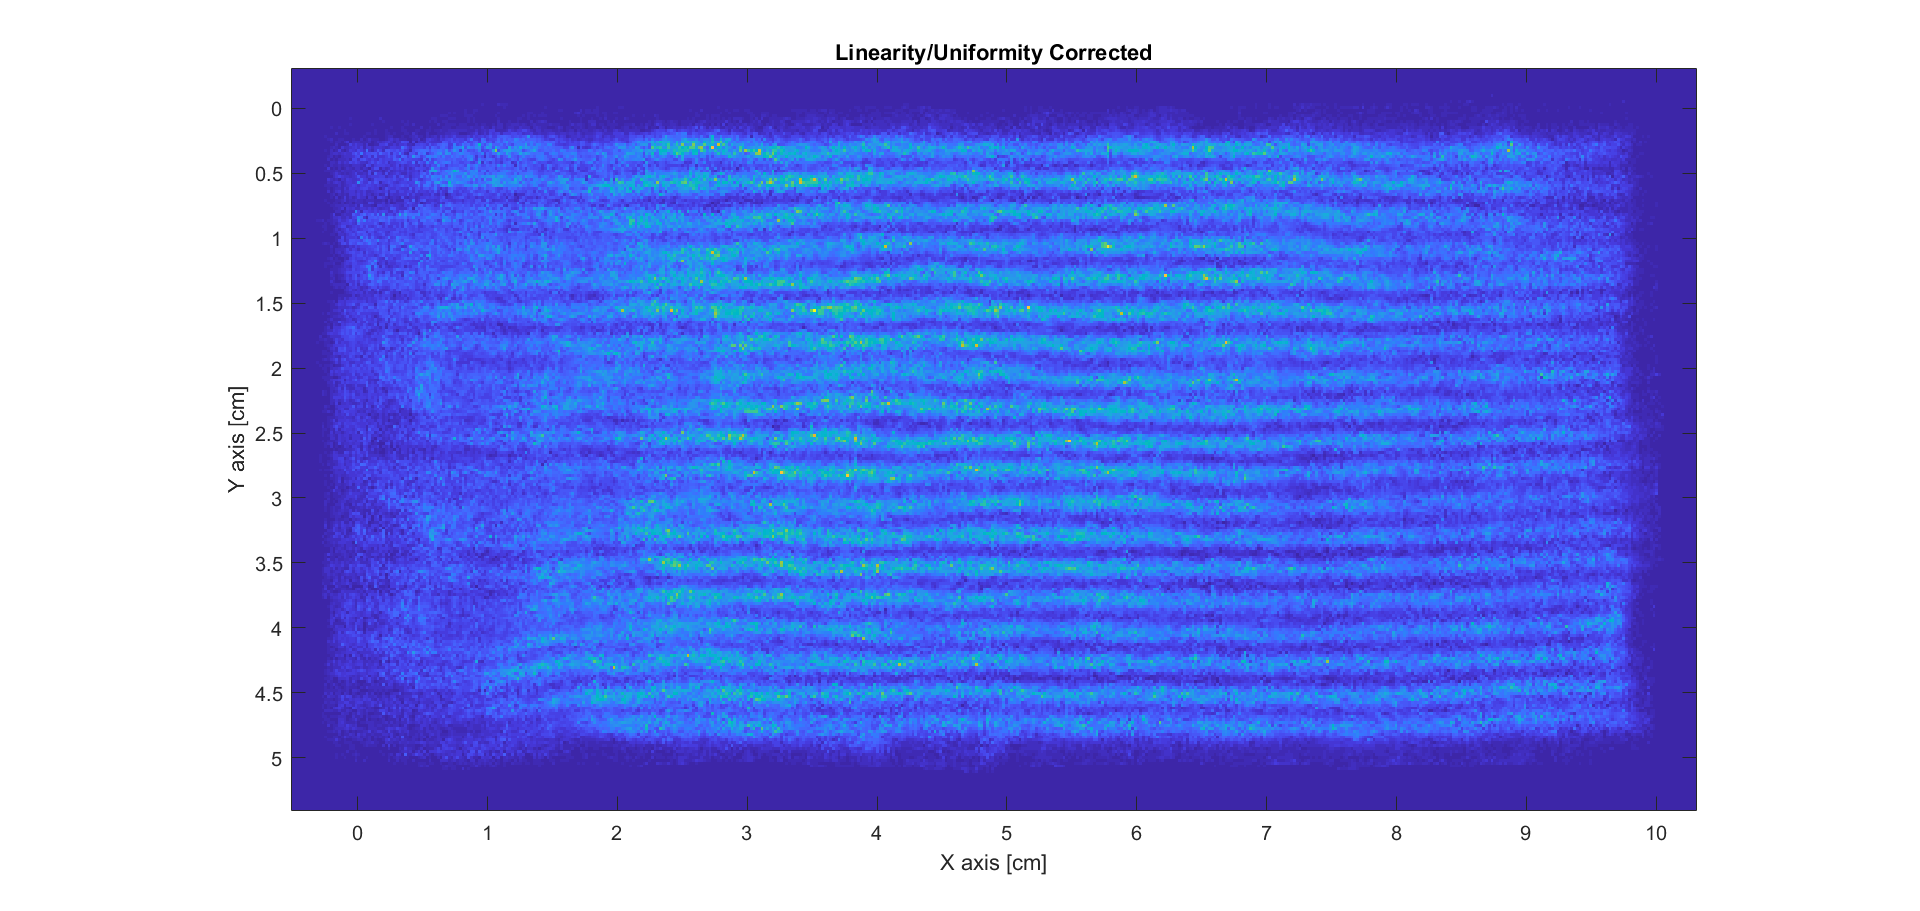
\includegraphics[width=0.8\textwidth]{figures/LondonLinCorr.png}\label{fig:wronglin}}
  \hfill
  \subfloat[The incorrect LRF is applied to this data ]{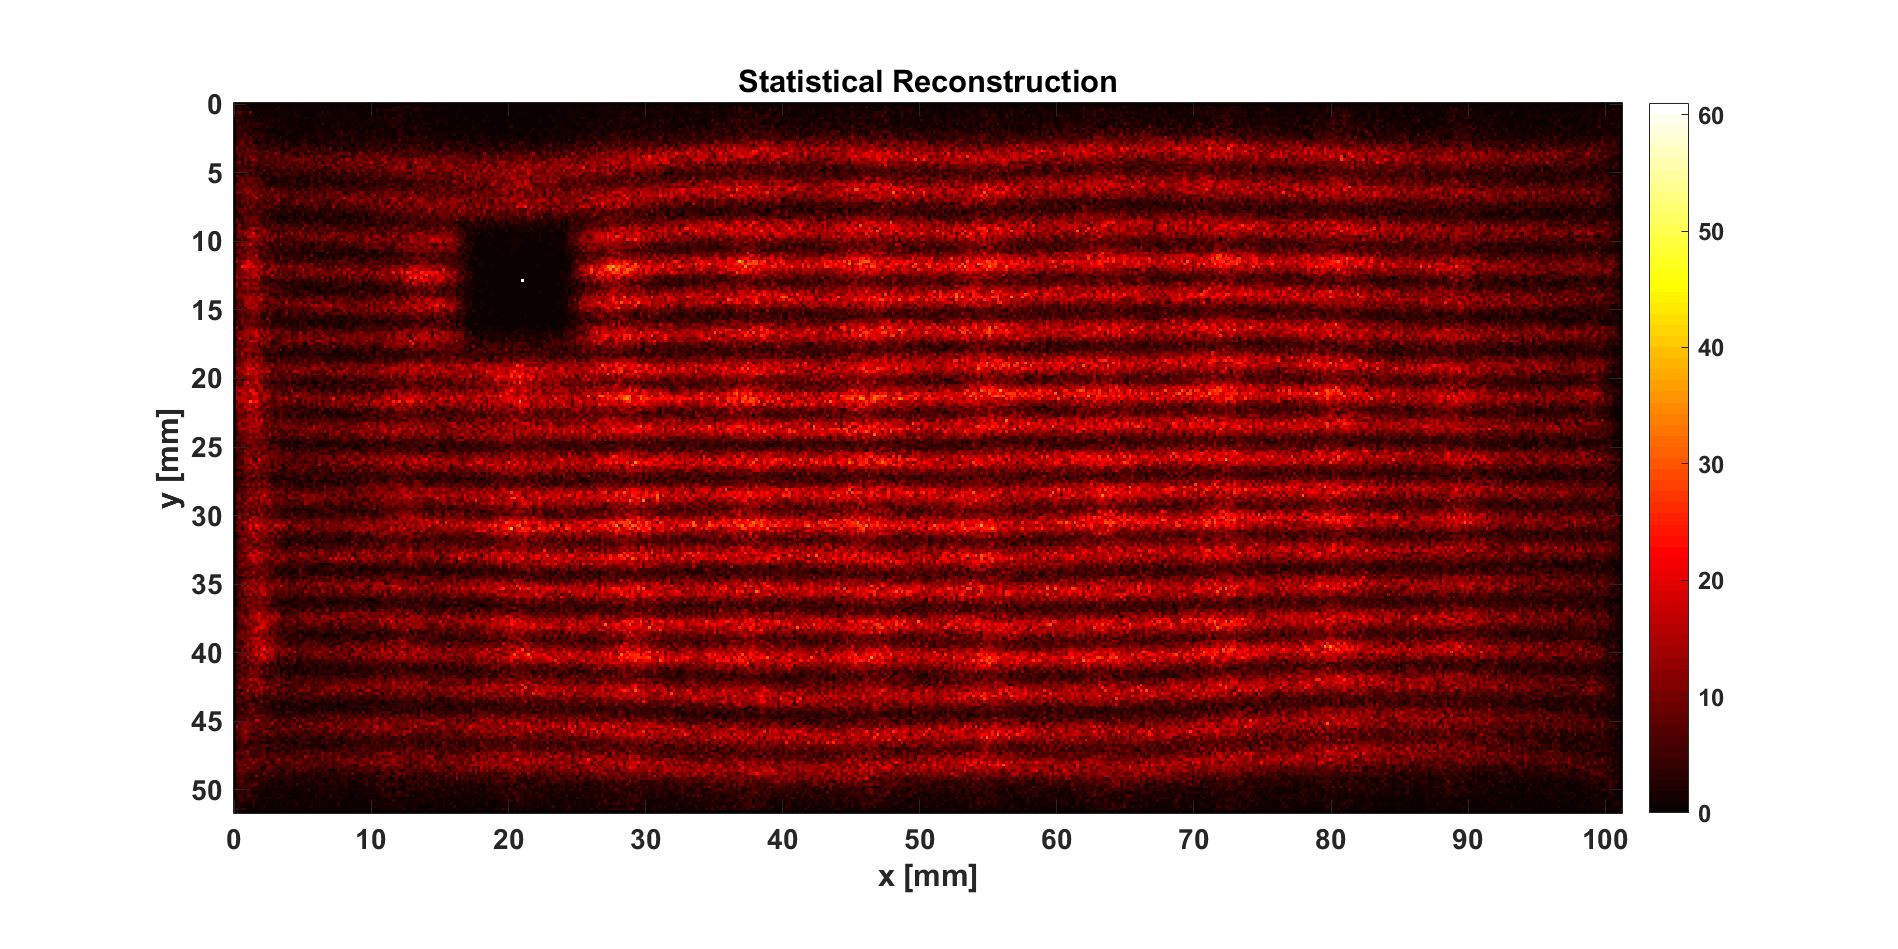
\includegraphics[width=0.8\textwidth]{figures/Node19wrongLRF.png}\label{fig:wrongLRF}}
  \caption{Without regular calibrations we cannot account for the instability in the detector modules.}
\end{figure}

The potential alternative linearity calibration would involve the use of capillary phantoms. This technique would be similar to the geometrical calibration, where the \acrshort{MSS} collimator is used when acquiring a series of horizontal and vertical capillaries \cite{Smith1988AcquisitionAnalysis}. The geometric and linearity calibration both involve a geometric transformation, carrying out these transformations simultaneously would be possible as the geometric distortion is minimal. The projects acquired from these phantoms would present a series of linear lines which can be modelled with the new software. This technique would reduce the time needed to carry out a linearity calibration as multiple detectors can acquire data at a time. In order to carry out this technique within the \acrshort{MR}, we would not be able to use the rotating motor, previously used to position the capillaries. An alternative would be to build a rotating frame or phantom to position the capillaries within the \acrshort{INSERT} \acrshort{FOV}.
\paragraph{}
The development of the calibration software also provides a means to implement an improved event reconstruction and image reconstruction algorithm. As discussed in chapter \ref{Linearity} an improved event reconstruction algorithm has been used to aid with linearity correction. This algorithm can be further improved and evaluated to create a complete pipeline for the reconstruction and calibration of the \acrshort{INSERT} data. Current work at Polimi aims to incorporate \acrshort{DOI} information within the reconstruction \cite{MASSARA2018ProcessingSystem}, this can be used to improve the existing image reconstruction. 

\section{SIMIND simulations}
Alternative procedures and designs, such as the calibration protocol, can be tested with Monte Carlo software. This would be a faster and cheaper method of testing proposed designed before they are implemented in the real system. Monte Carlo methods have proven successful for the evaluation of the \acrshort{INSERT} design in the past using GATE \cite{1236960} \cite{Busca2014SimulationImaging}.
\paragraph{}
SIMIND is a Monte Carlo software developed to simulate clinical imaging systems \cite{LJUNGBERG1989257}. The software provides the design for standard clinical simulations but also allows for the diverse modification of any experimental set up \cite{Gustafsson2018MonteFramework}. Michael Ljungberg developed SIMIND and has provided us with a prototype implementation of the clinical \acrshort{INSERT} scanner. This simulated environment would provide many possible experimental setups and allow us to test proposed design changes with no risk to the physical system. 
\paragraph{}
The \acrshort{INSERT} has been simulated before to great success, however, we moved to SIMIND as it promised a faster and more versatile software. The simulated \acrshort{INSERT} has not been fully tested and so future work with this system would require a complete implementation to ensure successful testing. 
\paragraph{}
\section{Contingency Plan}
SIMIND also offers the possibility to continue research in the event of a fatal error or malfunction within the system. Simulated work may be an option should we have a serious hardware failure or are unable to carry out further experiments. Though unlikely it is important to consider contingency plans if the system is unable to carry out the intended work within the clinical \acrshort{MRI}. The system can function as a stand-alone \acrshort{SPECT} scanner which is specialised to brain imaging. This could provide a useful analysis tool when studying conditions such as epilepsy. Studies in epilepsy would be particularly useful with the \acrshort{INSERT} as it is a portable system. It provides the possibility of bedside acquisitions and the ability to easily capture ictal and interictal images. The ability to bring the scanner to the patient would be very useful for many patients who are bed-bound and would be discomforted by being transported to a scanner. The \acrshort{INSERT} also provide relatively fast acquisitions, this could carry out standard investigations such as a DaTSCAN for the evaluation of Parkinson's disease. Should the system fail within the \acrshort{MR} we will consider our options and explore these alternative uses of the stand-alone \acrshort{SPECT}. 

\section{Clinical Studies}
To ensure the \acrshort{INSERT} can produce quality clinical \acrshort{SPECT} images we must compare it with existing technology. A phantom acquisition comparison of clinical \acrshort{SPECT} systems with the benchtop \acrshort{INSERT} will allow us to assess the imaging capabilities of the INSERT. A phantom acquisition can be carried out using the standard procedures from both systems. The results will indicate how the \acrshort{INSERT} can be improved to measure up to clinical \acrshort{SPECT}.
\paragraph{}
As a patient study is the final goal of the \acrshort{INSERT} we must also be able to compare the results of our simultaneous \acrshort{SPECT/MR} to that of the current clinical procedures. As it stands the combination of \acrshort{SPECT} and \acrshort{MRI} data is only possible with a \acrshort{SPECT/CT} system. The \acrshort{CT} provides a common anatomical mapping with the \acrshort{MR} which can be registered onto the \acrshort{SPECT} data. Acquiring this data and carrying out the comparison will determine the effective use of the \acrshort{INSERT}. 
\paragraph{}
The processing of these data will help develop a method of registration of the \acrshort{SPECT} and \acrshort{MR} images. An established method of combining this data to produce clinically useful images can be used within the \acrshort{INSERT}. These studies will also enable the preparation of the first in man studies with the \acrshort{INSERT}. Achieving comparable results with clinical systems will help establish ethical approval for the use of the novel \acrshort{SPECT} technology. 

\section{Clinical installation}
Before we look to patient trials, it is essential that we prove the completed \acrshort{SPECT/MRI} system can function. The next immediate goal of this work is to carry out the installation of the \acrshort{INSERT} within a clinical \acrshort{MRI}. This task is a major challenge as we must be able to safely incorporate each component of the \acrshort{INSERT} within the \acrshort{MR} environment. Following this installation, we must carry out extensive tests to ensure the mutual compatibility of the \acrshort{SPECT} and \acrshort{MRI}. To ensure no electromagnetic interference is encountered between the systems, mutual \acrshort{RF} shielding will be considered \cite{Lee2018LowApplications}. This sets out to protect the \acrshort{INSERT} from the \acrshort{RF} signals from the \acrshort{MR} as well as shield any noise from the \acrshort{INSERT} power supply \cite{Salvado2016ShieldingSystem}. This can be achieved by implementing techniques within \acrshort{PET/MR} \cite{Peng2014New7T} and preclinical \acrshort{SPECT/MR}.
\paragraph{}
The installation of the \acrshort{INSERT} within the \acrshort{MR} has begun. We have installed the system within the Macmillan Cancer Centre's \acrshort{PET/MR}. This facility is designed for radiation safety and so makes the installation easier as we can integrate the \acrshort{SPECT} with existing nuclear medicine support. The \acrshort{INSERT} scanner is designed for \acrshort{MR} compatibility but the external components are not. The cooling system and electrical control boards are not suitable within the \acrshort{MR} and so must be controlled from outside. This has been considered and a series of filter plates have been designed to allow the control of the \acrshort{INSERT} from outside of the \acrshort{MR} room. The use of novel technology within the clinic requires health and safety considerations to ensure all risks are assessed with regards to the technology and users. With the help of the \acrshort{UCH} \acrshort{MR} team, a `standards of practise' document has been created, which sets out the safe use of the \acrshort{INSERT} and considers the potential risks within the \acrshort{MR} environment. The document outlines the protocols which must be carried out, including the use of an \acrshort{MR} compatible trolley which has been designed specifically for the \acrshort{INSERT} scanner. Following our initial use of the scanner we established a need for an ergonomic collimator loading system, the trolley has been designed and built to ease the loading of the \acrshort{INSERT} and provide the safe use within the \acrshort{MR}. 
\paragraph{}
Once the installation is completed we set out to establish the first successful simultaneous scans of the \acrshort{SPECT/MRI}. A series of quality control and baseline measurements will be carried out to ensure the presence of the \acrshort{INSERT} has not affected the use of the \acrshort{MR}. Following this, we must ensure the \acrshort{MR} does not interfere with the \acrshort{INSERT}. Once mutual compatibility is achieved, we can continue with phantom studies; these will involve the assessment of the new calibration procedures, establishing phantom single and dual acquisitions, and optimising the \acrshort{MR} sequences used with the \acrshort{INSERT}. We will carry out a continuous technical validation of the system during any acquisition in or out of the \acrshort{MRI}. We must ensure stability, mutual compatibility and reproducibility. These will establish a safe and useful need of the system within patients and show an ethical study is viable. The risks and complications must be analysed thoroughly, the system design is not enough, we must also implement safety protocols to ensure risk is minimised and avoided. This may involve the production or purchase of safety equipment to aid in procedures and patient comfort. Once we can prove the safe and reproducible use of the complete \acrshort{INSERT} system, we can set out to achieve the first goal of the first patient scan in a clinical \acrshort{SPECT/MRI}.